% % % % % % % % % % % % % % % % % % % % % % % % % % % % % % % % % %
%  Devolutiva Final — Projeto Final (Módulo 3)
%  Grupo: EASE
%  Profa. Samara Silva · ETE Cícero Dias · Recife
% % % % % % % % % % % % % % % % % % % % % % % % % % % % % % % % % %

\documentclass[
  sigconf,
  nonacm,
  language=portuguese
]{acmart}

% ── Desliga rodapé ACM ──────────────────────────────────────
\settopmatter{printacmref=false}
\setcopyright{none}
\acmYear{2026}
\let\balance\relax

% ── Mata a página temporária da ACM (compilação única via API) ──
\makeatletter
\def\acm@addtemp@page{}
\makeatother

% ── Pacotes ─────────────────────────────────────────────────
\usepackage[portuguese]{babel}
\usepackage{microtype}
\usepackage{booktabs}
\usepackage{tabularx}
\usepackage{array}
\usepackage{colortbl}
\usepackage[dvipsnames,table]{xcolor}
\usepackage[inline]{enumitem}
\usepackage{graphicx}
\usepackage{adjustbox}
\usepackage{fancyhdr}
\usepackage{eso-pic}

% ── Ajuste contra quebras de texto ruins ────────────────────
\tolerance=1000
\emergencystretch=1.5em

% ── Cores ───────────────────────────────────────────────────
\definecolor{cgood}{HTML}{1E6B3A}
\definecolor{cwarn}{HTML}{8B4500}
\definecolor{cred}{HTML}{C0392B}
\definecolor{cmuted}{HTML}{666666}
\definecolor{crow}{HTML}{F2EFEB}

% ── Colunas customizadas ────────────────────────────────────
\newcolumntype{L}[1]{>{\raggedright\arraybackslash}p{#1}}
\newcolumntype{C}[1]{>{\centering\arraybackslash}p{#1}}

% ── Comandos ─────────────────────────────────────────────────
\newcommand{\notadestaque}[2]{%
  \noindent\textbf{Nota:}\enspace%
  {\large\bfseries\color{cred}#1\,/\,#2\,pts}%
}
\newcommand{\statusok}[1]{{\small\bfseries\color{cgood}#1}}
\newcommand{\statuswarn}[1]{{\small\bfseries\color{cwarn}#1}}
\newcommand{\gmax}[1]{{\color{cgood}\textbf{#1}}}
\newcommand{\gcut}[1]{{\color{cwarn}\textbf{#1}}}

% ── Renomeações PT-BR ────────────────────────────────────────
\AtBeginDocument{%
  \renewcommand{\abstractname}{Resumo}
  \renewcommand{\figurename}{Figura}
  \renewcommand{\tablename}{Tabela}
}

% ────────────────────────────────────────────────────────────
\begin{document}

% ── CAPA ────────────────────────────────────────────────────
\thispagestyle{empty}
\AddToShipoutPictureBG*{%
  \AtPageLowerLeft{%
    \IfFileExists{capa-ease.png}{%
      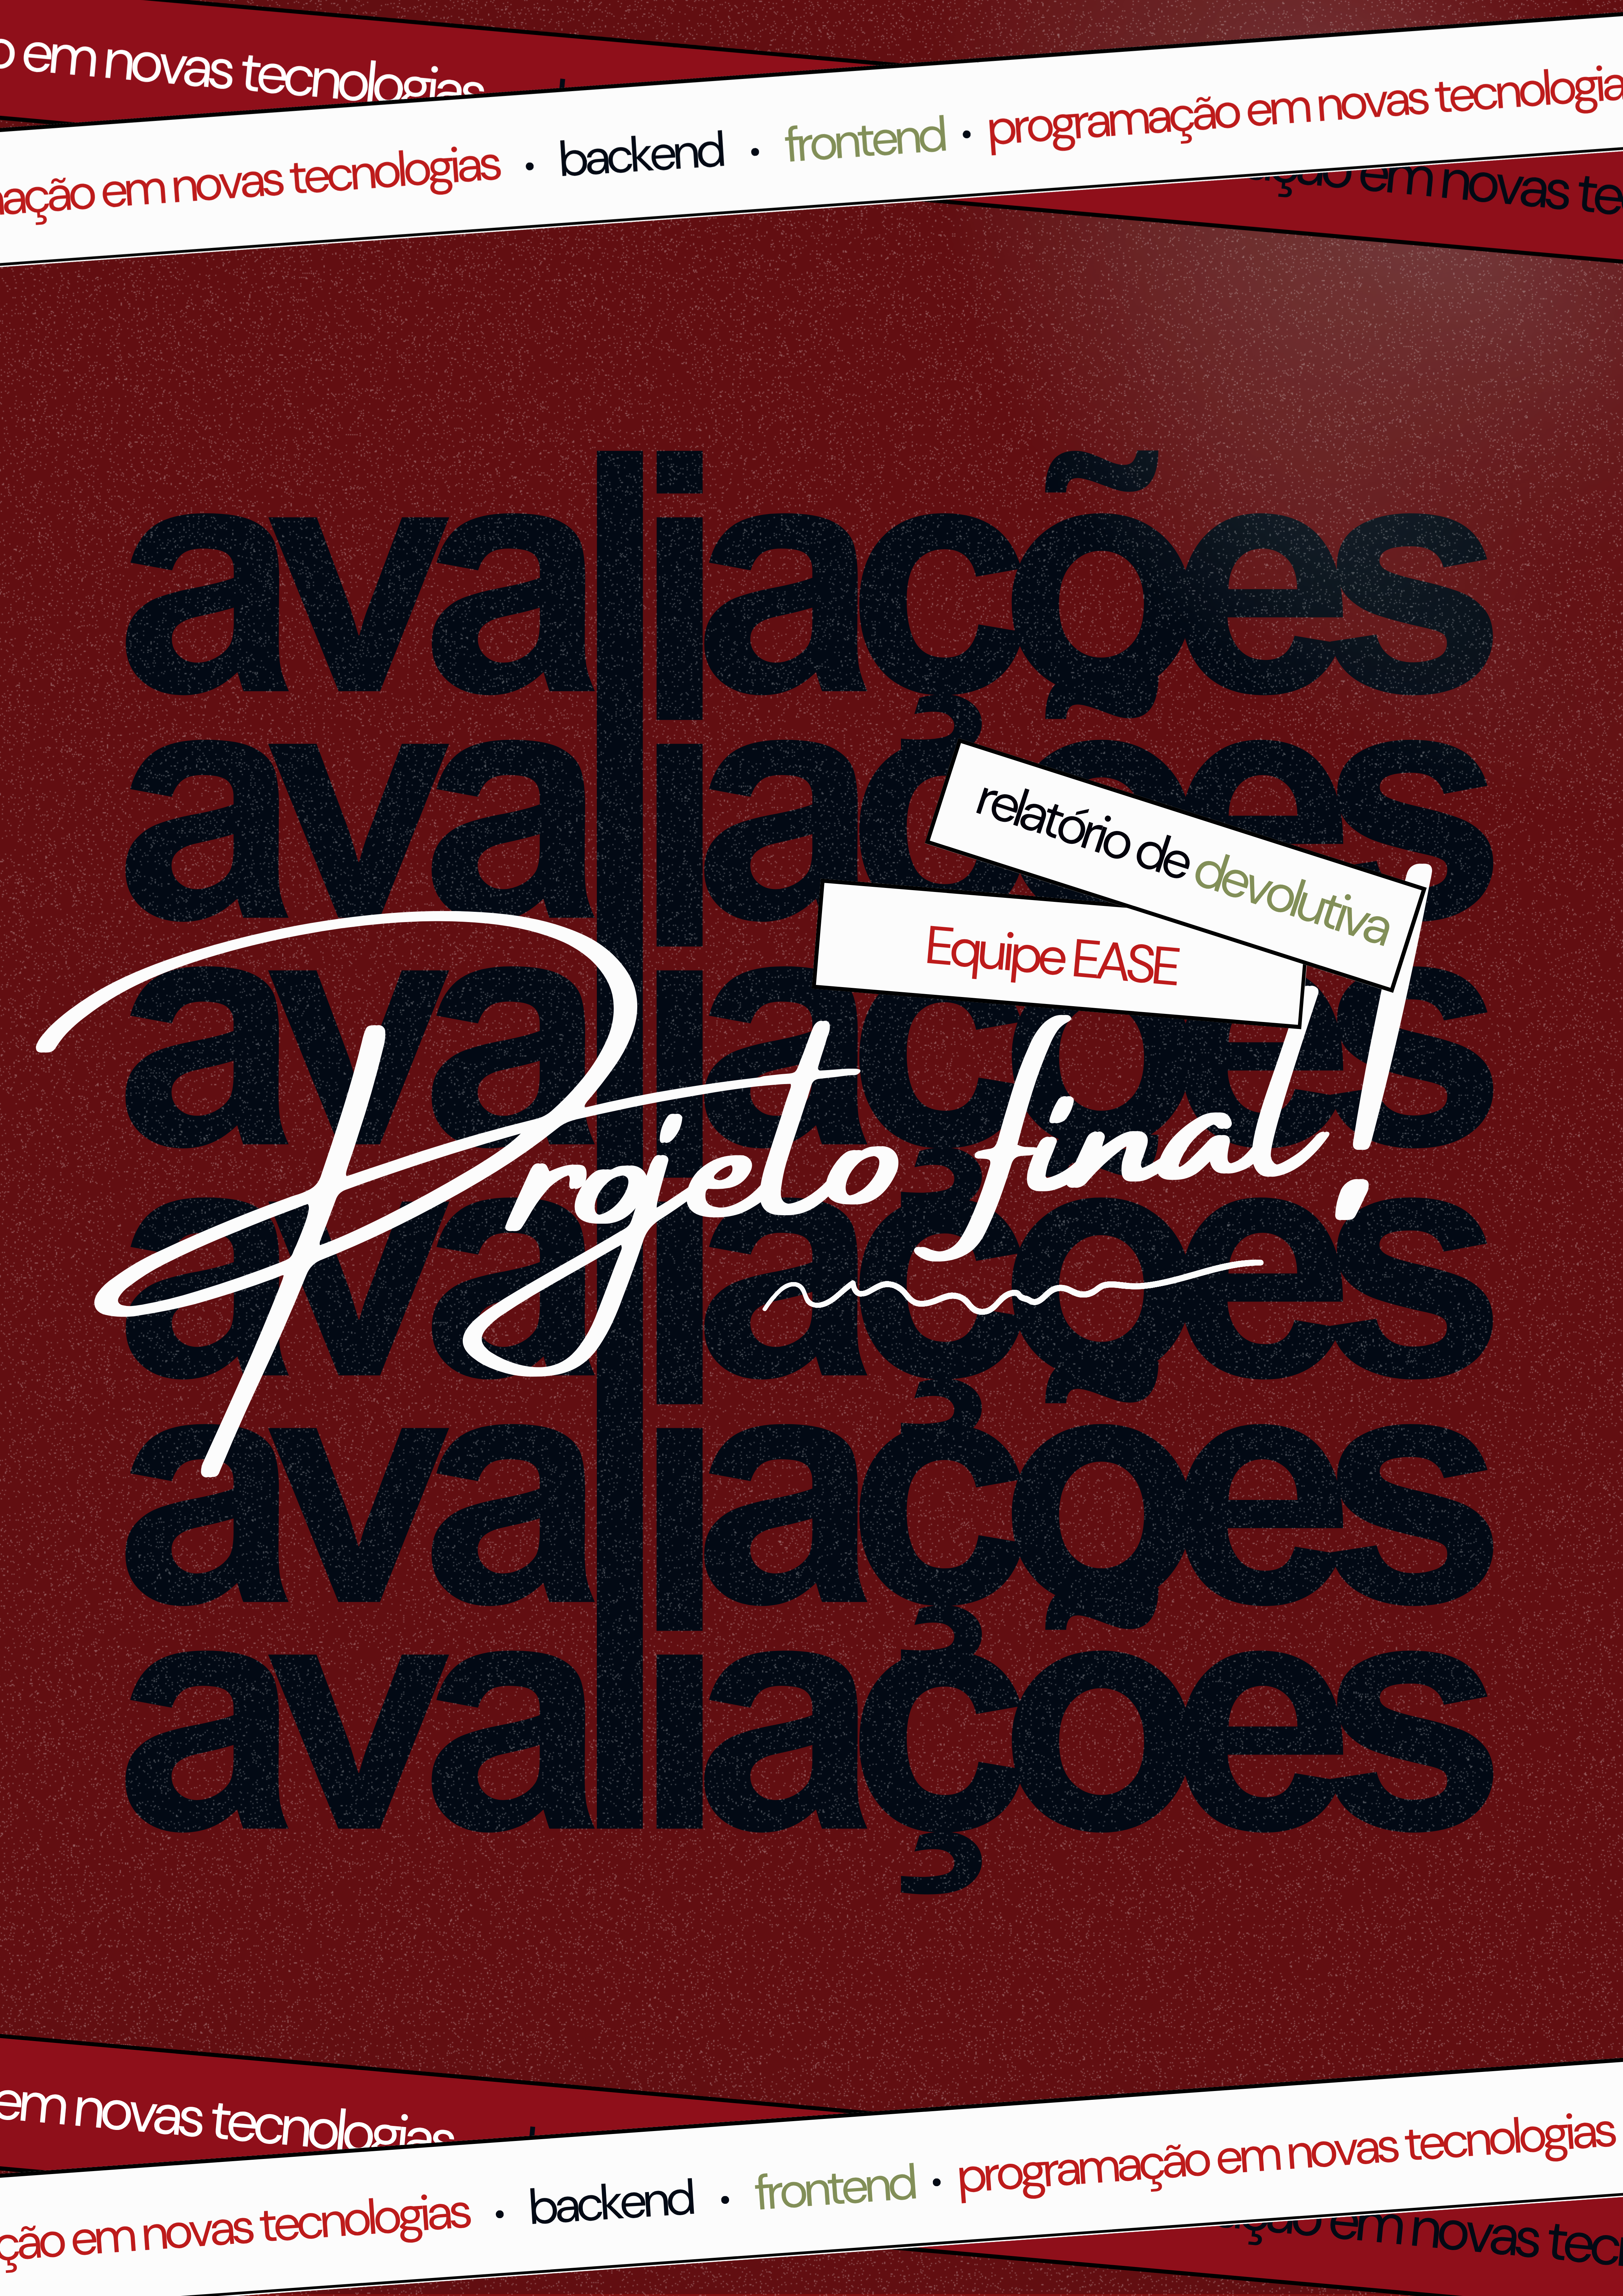
\includegraphics[width=\paperwidth,height=\paperheight]{capa-ease.png}%
    }{%
      \IfFileExists{../../capa-ease.png}{%
        
\includegraphics[width=\paperwidth,height=\paperheight]{../../capa-ease.png}%
      }{%
        \parbox[b][\paperheight]{\paperwidth}{%
          \vspace*{10cm}\begin{center}{\large\color{gray}[capa-ease.png não encontrada]}\end{center}%
        }%
      }%
    }%
  }%
}
\mbox{}
\clearpage

% ── CONFIGURAÇÃO DE PÁGINA PÓS-CAPA ─────────────────────────
\setcounter{page}{1}
\pagestyle{fancy}
\fancyhf{}
\renewcommand{\headrulewidth}{0pt}
\fancyfoot[C]{\thepage}
\setlength{\headsep}{0.8cm}

% ── METADADOS ────────────────────────────────────────────────
\title{Feedback Avaliativo de Projeto: Projeto Final --- EASE}

\author{Profa.\ Samara Silva}
\authornote{Grupo: \textbf{EASE} \textperiodcentered\ M\'{o}dulo 3 --- Projeto Final \textperiodcentered\ Avaliado em: 18 de junho de 2026.}
\email{samarasilvia.educa@gmail.com}
\affiliation{%
  \institution{ETE C\'{i}cero Dias}
  \department{M\'{o}dulo 3 --- Programa\c{c}\~{a}o em Novas Tecnologias · 2026.1}
  \city{Recife}
  \state{Pernambuco}
  \country{Brasil}
}

\author{EASE}
\affiliation{%
  \institution{ETE C\'{i}cero Dias}
  \department{Cybele · Levi · Roberta · William}
  \city{Recife}
  \state{Pernambuco}
  \country{Brasil}
}
\maketitle

\vspace{1em}
\section{Avaliação Geral}

A avaliação do Projeto Final foi concluída. A seguir, o resumo dos critérios, os comentários detalhados e a grade completa da apresentação.

\subsection{Resumo dos Critérios}

{\small
\rowcolors{2}{crow}{white}
\begin{tabularx}{\linewidth}{@{} >{\raggedright\arraybackslash}X c c c @{}}
\toprule
\textbf{Critério} & \textbf{Status} & \textbf{Nota} & \textbf{Máx.} \\
\midrule
AT1 --- Desempenho em sala & \statuswarn{Com ressalvas} & \textbf{2,2} & 3,0 \\
AT2 --- Documentação & \statusok{Completo} & \textbf{3,0} & 3,0 \\
AT3 --- Apresentação & \statuswarn{Com ressalvas} & \textbf{3,6} & 4,0 \\
\midrule
\textbf{1ª Nota (AT1+AT2+AT3)} & & \textbf{\color{cred}8,8} & \textbf{10,0} \\
2ª Nota --- Projeto Final & \statusok{Completo} & \textbf{10,0} & 10,0 \\
\bottomrule
\end{tabularx}}

\section{Comentários por Critério}

\subsection{Desempenho em sala}
\noindent\statuswarn{2,20\,/\,3,00 pts · Com ressalvas}

O engajamento e a participação do grupo no acompanhamento do projeto foram bons, mas houve inconsistência na frequência ao longo das aulas, o que reduziu a pontuação coletiva neste critério. A Roberta faltou praticamente todas as aulas, então zerou em desempenho (componente individual).

\subsection{Documentação}
\noindent\statusok{3,00\,/\,3,00 pts · Completo}

Documentação completa e adequada. Sem ressalvas.

\subsection{Apresentação}
\noindent\statuswarn{3,60\,/\,4,00 pts · Com ressalvas}

Na apresentação do EASE, eu particularmente não gostei que a Cybele não soube navegar bem no site, o que me deu uma certa impressão de falta de domínio: quando pediram para voltar à página original, ela não sabia onde estava o botão. Por isso tirei 0,4 décimos.

\par\medskip\noindent\textbf{Grade da Apresentação}\par\smallskip

{\small
\rowcolors{2}{crow}{white}
\begin{tabularx}{\linewidth}{@{} >{\raggedright\arraybackslash}X c c @{}}
\toprule
\textbf{Critério avaliado} & \textbf{Peso} & \textbf{Nota} \\
\midrule
Motivação & 0,15 & \gmax{0,15} \\
Desenvoltura no discurso & 0,40 & \gmax{0,40} \\
Postura & 0,25 & \gmax{0,25} \\
Funcionalidades & 0,40 & \gmax{0,40} \\
Design Centrado no Usuário & 0,40 & \gmax{0,40} \\
Escopo do Projeto & 0,25 & \gmax{0,25} \\
Tecnologia e Infraestrutura & 0,25 & \gmax{0,25} \\
Roadmap & 0,15 & \gmax{0,15} \\
Usabilidade & 0,40 & \gcut{0,20} \\
Responsividade & 0,15 & \gmax{0,15} \\
Fluxo das Tasks & 0,25 & \gmax{0,25} \\
Domínio no tema & 0,40 & \gcut{0,20} \\
Inovação/Diferencial Competitivo & 0,15 & \gmax{0,15} \\
Deu tempo de falar tudo & 0,15 & \gmax{0,15} \\
Casos de uso & 0,25 & \gmax{0,25} \\
\midrule
\textbf{Total} & \textbf{4,00} & \textbf{\color{cred}3,60} \\
\bottomrule
\end{tabularx}}

\vspace{2pt}
\noindent{\footnotesize\itshape Tempo de apresentação: 5 min.}\par
\noindent{\footnotesize Pesos por critério --- Alto: 0,40 · Médio: 0,25 · Baixo: 0,15 (somam 4,00).}

\subsection{Projeto Final}
\noindent\statusok{10,00\,/\,10,00 pts · Completo}

Entrega excelente.

\section{Considerações Finais}

Um ótimo trabalho no geral. Fica a recomendação de reforçar o domínio da navegação do próprio produto para as demonstrações ao vivo em apresentações futuras. Continuem assim!

% ── Assinatura ───────────────────────────────────────────────
\vspace{1.5em}
\noindent\rule{\linewidth}{0.4pt}

\begin{flushright}
\textbf{Profa.\ Samara Silva}\\
{\small\color{cmuted} Programação em Novas Tecnologias --- Módulo 3 · ETE Cícero Dias}\\
{\small\color{cmuted} Recife, 18 de junho de 2026}
\end{flushright}

% ── Notas por integrante ─────────────────────────────────────
\appendix
\onecolumn
\section{Notas por Integrante}

A média final consolida o desempenho em sala, a documentação, a apresentação e o projeto final. Descontos individuais por frequência são aplicados sobre a nota do grupo.

\vspace{0.5em}
\begin{tabularx}{\linewidth}{@{} X p{3cm} p{2.5cm} @{}}
\toprule
\textbf{Integrante} & \textbf{Observação} & \textbf{Média Final} \\
\midrule
Cybele & --- & \textbf{9,5} \\
Levi & --- & \textbf{9,5} \\
William & --- & \textbf{9,5} \\
Roberta & Zerou em desempenho (faltas) & \textbf{8,5} \\
\bottomrule
\end{tabularx}

\end{document}